\documentclass[a4paper]{article}

%use the english line for english reports
%usepackage[english]{babel}
\usepackage[portuguese]{babel}
\usepackage[utf8]{inputenc}
\usepackage{indentfirst}
\usepackage{graphicx}
\usepackage{verbatim}
\usepackage{color}
\usepackage{indentfirst}
\usepackage{listings}
\usepackage[utf8]{inputenc}
\usepackage{biblatex}
\usepackage{appendix}

\begin{document}

\setlength{\textwidth}{16cm}
\setlength{\textheight}{22cm}

\title{\Huge\textbf{Plano de Negócios}\linebreak\linebreak\linebreak
%\Large\textbf{Apresentação da Empresa}\linebreak\linebreak
\linebreak\linebreak

\includegraphics[scale=0.1]{feup-logo.png}\linebreak\linebreak
\linebreak\linebreak
\Large{Mestrado Integrado em Engenharia Informática e Computação} \linebreak\linebreak
\Large{Análise de Projetos de Investimento}\linebreak
}

\author{\textbf{Grupo 03:}\\
Duarte Manuel Marques Mano Menezes Frazão - 201605658 \\
Fábio Manuel Neves de Araújo - 201607944 \\
Francisco Teixeira Ferreira - 201605660 \\
João Carlos Fonseca Pina de Lemos - 201000660 \\
João Miguel Vaz Tello da Gama Amaral - 201708805 \\
João Nuno Rodrigues Ferreira - 201605330\\\linebreak\linebreak \\
 \\ Faculdade de Engenharia da Universidade do Porto \\ Rua Roberto Frias, s\/n, 4200-465 Porto, Portugal \linebreak\linebreak\linebreak
\linebreak\linebreak\vspace{1cm}}
%\date{Junho de 2007}
\maketitle
\thispagestyle{empty}

%************************************************************************************************
%************************************************************************************************

\newpage


\tableofcontents

%************************************************************************************************
%************************************************************************************************

%*************************************************************************************************
%************************************************************************************************

\newpage

%%%%%%%%%%%%%%%%%%%%%%%%%%
%Sintese histórica%
\part{Sumário executivo}
O presente Plano de Negócios visa avaliar o método de criação e funcionanemnto da empresa Nanawave para o períudo compreendido entre os anos 2021-2026. Tendo em conta o estadado atual da economia mundial e às dificuldades acrescidas da pandemia, foi decidido adiar o começo do plano pra o fim do 2º trimestre do primeiro ano do projeto. A questão central que se quer responder decorre da avaliação económico-financeira realizada neste plano, no sentido de aferir se a ideia de negócio se demonstra lucrativa no prazo apresentado de forma a poder ser apresentado em reuniões de investimento.

\part{Apresentação empresa}

\includegraphics[scale=1]{LOGO.png}

%Sintese histórica%
\section{Apresentação do histórico}
\subsection{Produto}
NanoWave é um microondas portátil com bateria, desenvolvido para levar em viagens, passeios, ou em situações do dia-a-dia em que necessitemos de aquecer comida sem ou escasso acesso a um microondas.
\subsubsection{Mercado Alvo}
O nosso mercado alvo tem um foco em dois grupos de consumidores:
\begin{itemize}
    \item Viajantes casuais que queiram aquecer comida numa viagem, passeio ou piquenique
    \item Trabalhadores que optem por levar comida de casa para comer no trabalho, sem acesso a microondas ou de utilização incómoda (filas)
\end{itemize}

\subsection{Concorrentes}
\begin{itemize}
    \item Microondas portátil com isqueiro de carro
    \item Equipamentos de aquecimento de campismo a gás
    \item Equipamentos de aquecimento de campismo a luz solar
    \item Equipamentos de aquecimento de campismo a eletricidade
\end{itemize}

\subsection{Fornecedores principais}
De modo a construir o nosso produto iremos começar por apenas fazer a montagem e design do produto in-house e dar outsource da manufatura das peças.\\
No ínicio teríamos os seguintes possíveis fornecedores:
\begin{itemize}
    \item DuarteCruz Fábrica de Plásticos Lda - Plásticos para a estrutura do produto
    \item Energia lateral - Tecnologia microondas microondas
    \item Only Battery - Bateria do produto
\end{itemize}

\section{Missão, objetivos e desafios futuros}
A nossa missão é, através de soluções mais ágeis, conseguir apoiar as pessoas, tornando as suas vidas mais práticas. Atendendo às grandes necessidades das pessoas se movimentarem bastante, tanto a nível profissional com pessoal, queremos conseguir tornar o seu dia a dia, o mais confortável possível.\\
Pretendemos conquistar o maior número de clientes no nosso mercado nacional e conseguir expandi-lo para o estrangeiro, por meio de parcerias com os maiores retalhistas que já existem a nível mundial. Também ambicionamos o mercado online, fazendo do mesmo modo chegar os nossos produtos aos nossos clientes.\\
O nosso objetivo é trazer a comodidade de equipamentos domésticos mas com portabilidade.

\section{Planeamento estratégico e implementação}
O desenvolvimento da NanoWave passa por divulgar o produto já existente, criando também outras gamas do mesmo produto para responder a várias necessidades. O desenvolvimento do produto é da responsabilidade equipa de R\&D que passa os designs para a equipa responsável pela manufatura (inicialmente outsourced) e montagem do produto.\\
Preocupamo-nos por garantir a competividade dos nossos produtos no mercado tendo em conta os seguintes pontos:\\
\begin{itemize}
 \item Preço
 \item Know how dos nossos recursos humanos
 \item Estabelecimento de uma relação de proximidade e confiança com o cliente
 \item Relações de integridade para com os fornecedores
 \item Serviço pós-venda com um grau elevado de satisfação
 \item Flexibilidade para compreender os clientes e ajustar a oferta às verdadeiras necessidades
 \item Desenvolvimento de produtos com um estilo próprio, com características especiais, com elevada durabilidade e com um desempenho excecional
\end{itemize}

A nível de Marketing apostaremos fortemente no marketing digital, sendo esta a principal fonte dos nossos rendimentos. Vamos usar publicidade quer através de anúncios pagos em redes sociais quer através do patrocínio de influencers que trazem tráfego para página online da NanoWave onde a compra é finalizada.

\section{Estrutura Legal}
No que diz respeito à estrutura legal da empresa, esta será uma sociedade limitada constituída por 6 membros fundadores com uma divisão igualmente repartida das quotas, contribuindo para que cada sócio tenha uma percentagem de controlo da empresa de aproximadamente 17\%, sendo que em caso de distribuição do capital da organização, quando esse mesmo montante não é investido, cada membro recebe essa mesma percentagem do lucro obtido pela empresa.\\
O facto de ser uma sociedade limitada faz com que a responsabilidade de cada sócio seja restrita à empresa, sendo que os bens pessoais de cada membro são protegidos em caso de falência. Em caso de prejuízo, há uma proibição da distribuição dos lucros da empresa para os sócios, sendo que a sociedade limitada tem como objetivo principal garantir a estabilidade da organização. Dada esta prioridade em garantir a manutenção da empresa, este tipo de estrutura legal constitui um incentivo ao investimento externo.

\section{Parcerias}
As parcerias a estabelecer são um ponto importante que deve ser altamente valorizado de modo a promover a entrada do produto no mercado e aumentar as respectivas vendas.\\
Visto que o nosso produto apenas funciona com tupperwares de certas dimensões, uma das parcerias que poderia ser estabelecida seria com a Tupperware Brands Corporation. A Tupperware é a principal marca da empresa Tupperware Brands Corporation, indústria especializada em produtos de plástico, especialmente recipientes para utilização na conservação e preparação de alimentos. A parceria teria como objetivo responsabilizar a Tupperware pela produção dos recipientes a utilizar com o NanoWave.\\
Estabelecer uma parceria com uma empresa distinguível nesta área é uma mais valia na divulgação e reconhecimento do produto.

\section{Equipa de Gestão}
A empresa será composta por CEO, Gestor de Marketing e Vendas, Gestor de Stocks e um Encarregado de Montagem e de Qualidade e todo o restante pessoal para a montagem do produto. O CEO será responsável por manter o correto funcionamento da empresa e a interligação entre todos os departamentos, o Gestor de Marketing e Vendas vai ter que divulgar o nosso produto de forma eficiente e controlar as vendas e a sua evolução, o Gestor de Stocks irá assegurar sempre a existência de materias para que a montagem dos NanoWaves seja feita com sucesso e com qualidade e o Encarregado de Montagem irá assegurar a correta montagem dos produtos e também a sua qualidade e o seu funcionamento.

\section{Responsabilidade Social}
A responsabilidade social é algo que é tido em grande consideração na tomada de decisões desta sociedade. Isto porque, de facto, acreditamos que podemos aliar os resultados financeiros fundamentais à nossa estabilidade e ao impacto positivo que podemos ter, tanto na nossa equipa e nos nossos clientes, como no meio ambiente.\\
Dito isto, caracterizamo-nos por apresentar uma responsabilidade social corporativa, com esforços constantes na melhoria do ambiente de trabalho da equipa e na solidificação das relações interpessoais entre todos os constituintes da empresa, visando também promover a saúde de todos os colaboradores, para lá do legalmente exigido. Para além disto apresentamos ainda uma forte responsabilidade ambiental, com o intuito de minimizar o consumo de recursos, nomeadamente de energia elétrica, não só na fase de produção mas também durante o próprio consumo do utilizador.


\part{Apresentação produto/serviço}
O NanoWave combina o design tradicional e funcional de um microondas com a facilidade de portabilidade que um item portátil merece. Com um design simples rectangular cabe facilmente na bolsa de transporte, tendo capacidade para aquecer um recipiente de alimentos de cada vez.\\
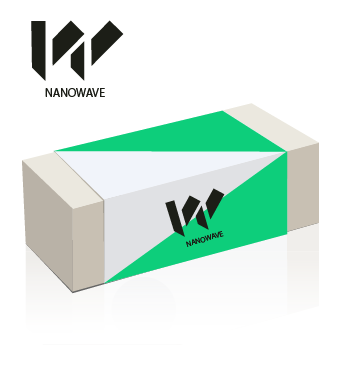
\includegraphics[scale=0.5]{package.png}

\section{Principais Utilizações}
NanoWave traz a comodidade do microondas a lugares onde antes não o era possível utilizar como podemos verificar pelas seguintes possíveis utilizações do produto:
\begin{itemize}
    \item Um trabalhador ou estudante que opte por trazer comida de casa muitas vezes depara-se com um dos seguintes problemas:
    \begin{enumerate}
        \item Não existe um microondas disponível
        \item Existe microondas mas, sendo partilhado, tem de se esperar numa fila para que outras pessoas aqueçam primeiro a sua comida, sendo também difícil garantir uma boa higiene desse microondas
    \end{enumerate}
    \item Famílias que façam viagens ou piqueniques em parques beneficiariam de ter acesso a um equipamento que aquecesse comida ou bebida, uma vez que a maior parte das vezes não terão acesso a eletricidade e o carro estará longe do local (por exemplo no parque)
\end{itemize}

\section{Produtos complementares e substitutos existentes}
Em relação aos produtos complementares foram identificados:
\begin{itemize}
    \item Recipientes de plástico ou vidro para conservar e preparar refeições como, por exemplo, Tupperwares
    \item Formas de transporte do NanoWave como uma mochila
\end{itemize}
Já em relação aos substitutos existentes:
\begin{itemize}
    \item Microondas portátil com isqueiro de carro
    \item Fogões de campismo portáteis elétricos
    \item Fogões de campismo a gás
    \item Fogões de campismo movidos a luz solar
\end{itemize}
\section{Vantagens competitivas face aos produtos concorrentes}
\begin{itemize}
    \item Utilização fixa ou portátil (devido à bateria)
    \item Alta portabilidade
    \item Bateria com durabilidade suficiente para uso regular no exterior
    \item Recarregável com cabo USB-C
\end{itemize}

\section{Fase de vida do produto}
A fase ou ciclo de vida do produto é um modelo que divide a linha de produção deste em 4 fases, que são: introdução, crescimento, maturidade e declínio.\\
Consideramos que, tanto na introdução como no crescimento do NanoWave, o investimento em publicidade deverá ser relativamente elevado, visto que é um produto novo que ainda tem que ganhar o seu espaço no mercado.\\
Quando se fala no período de maturidade do produto, é importante ter em consideração o preço praticado. Pensamos que deverá manter-se um preço modesto e acessível à maior parte do público alvo.\\
Por fim, devemos sempre ter em conta novos produtos ou formas de tornar o NanoWave mais atrativo de modo a que, durante o declínio do NanoWave, a nossa empresa esteja preparada para se manter competitiva em relação à concorrência.
\part{Plano de Marketing}
\section{Análise de Mercado}
\subsection{Análise do Setor}
\subsubsection{Mercado Alvo}
O principal mercado alvo no NanoWave são os pessoas que pretendam trazer comida de casa e aquecê-la mas que a utilização de um microondas seja impossível ou incómoda.
\subsubsection{Segmentação}
Este mercado-alvo divide-se em dois segmentos, nas empresas e em atividades na natureza.\\
No caso de empresas com um tamanho considerável a proporção de microondas para o número de colaboradores é muito baixa, criando filas grandes e no caso dos equipamentos não terem a manutenção devida e uma segurança alimentar duvidosa. Estudos também revelam que com o aumento da pressão de produtividade e performance nas empresas os colaboradores cada vez mais optam por comer a refeição na secretária de trabalho, sendo que nesse estudo 52\% de trabalhadores traz a comida de casa. Outra mercado ainda dentro das empresas são trabalhos de construção, onde não existe possibilidade de ter um microondas. \\
No caso das atividades na natureza, são pessoas que pretendem reaquecer comida em diversas atividades, seja caminhadas por parques ou no campismo, onde até agora apenas é possível usando um fogão a gás ou no carro.
\subsubsection{Dimensão do mercado}
De modo a calcular a dimensão total do mercado iremos fazer uma divisão pelos dois segmentos.

\textbf{Empresas:} De modo a estimar a dimensão do mercado de segmento das empresas optámos por usar a percentagem de pessoas que trabalha em portugal em serviços, assumindo que estas pessoas trabalham todas em ambientes onde o nosso produto fosse ser benéfico, de seguida aplicamos a estatística que referimos anteriormente sobre o número de pessoas que leva comida para o trabalho. Sendo assim no segmento empresas a nossa dimensão do mercado seria:\\
2 850 000 (pessoas que trabalham nos serviços) * 0.52 (pessoas que levam comida para o trabalho) 130 * (preço do NanoWave)=  192 660 000 euros \linebreak\linebreak
\textbf{Atividades na natureza:} De modo a estimar a dimensão de mercado do segmento atividades na natureza optámos por usar a percentagem de pessoas que faz caminhadas de montanha nos estados unidos (14\%) e aplicar à população de portugal (uma vez que Portugal não tem essa informação disponível). \\
10 280 000 (população portugal) * 0.14 * 130 (preço do NanoWave) = 187 096 000 \linebreak\linebreak
\textbf{Total:} Sendo assim podemos concluir que a dimensão do mercado no segmento das empresas é 192 milhões e nas atividades de natureza é 187 milhões. 
\subsubsection{Objetivos}
O objetivo no nosso produto é penetrar o mercado estagnado do aquecimento portátil e:
\begin{itemize}
 \item Eliminar tempos de espera em filas ou possibilitar o acesso a um microondas para colaboradores de empresa
 \item Auxiliar pessoas em atividades na natureza a conseguir ter refeições quentes
\end{itemize}

\subsection{Análise dos clientes potenciais}
Temos dois tipos de clientes.\\
Em primeiro lugar colaboradores de empresas que tenham trabalhos de escritório, tragam comida de casa e que beneficiem de perder menos tempo nas filas de microondas (se este existir). As necessidades destes clientes serão que o produto:
\begin{itemize}
    \item Seja portátil e discreto, de modo a caber em locais como um cacifo, debaixo da mesa, ou numa pequena mala do produto
    \item Tenha potência suficiente para realizar as refeições que o colaborador fizer num dia e que depois se possa carregar a bateria
\end{itemize}

Em segundo lugar pessoas que regularmente façam campismo ou piqueniques em parques e que beneficiem de ter a comida aquecida sem ter de trazer um fogão a gás. Também juntamos a este grupo os trabalhos de construção uma vez que as necessidades são as mesmas.
As necessidades destes clientes serão que o produto:
\begin{itemize}
    \item Seja portátil de modo a caber numa mochila e conseguir guardar os tupperwares da comida dentro do equipamento e poupar espaço
    \item Tenha potência suficiente para realizar as refeições que a pessoa necessite numa atividade na natureza 
    \item O equipamento deve ser resistente a vibrações que possam acontecer durante a caminhada
\end{itemize}


Relativamente às empresas, uma vez que possíveis clientes possam ser pessoas com mais possibilidades, uma versão mais cara que invista num design moderno poderá ser uma hipótese a ser explorada.\\
Outras hipóteses de variações de produto, mais viradas para a natureza, é um equipamento mais resistente para ser transportado em caminhadas ou então um produto mais direcionado à família, onde seria vendido com uma bateria de capacidade superior.

\subsection{Análise dos concorrentes}
Após análise da concorrência selecionamos os seguintes produtos:
\begin{itemize}
    \item Hotlogic
    \item Travelisimo
    \item Campingaz
\end{itemize}

Analisamos de seguida como o NanoWave se compara com estes três em diferentes categorias:

\subsubsection{Base de concorrência}
\begin{itemize}
    \item Hotlogic - Um aquecedor de comida portátil, a diferença principal para o NanoWave é o facto de funcionar com resistências em vez de microondas
    \item Travelisimo - Um aquecedor de comida portátil, a diferença principal para o NanoWave é o facto de ser alimentado por uma ligação ao isqueiro do carro
    \item Campingaz - Marca líder em fogões de campismo a gás, principal concorrente do NanoWave em atividades de natureza com a sua versão mais compacta
\end{itemize}

\subsubsection{Preço}
\begin{itemize}
    \item Hotlogic - 40\$
    \item Travelisimo - 30\$
    \item Campingaz - 20\$ + botijas de gás (5\$)
    \item NanoWave -  130\$
\end{itemize}

\subsubsection{Design}
\begin{itemize}
    \item Hotlogic - Aquecimento com resistência 
    \item Travelisimo - Aquecimento com resistência
    \item Campingaz - Aquecimento com gás, necessita de substituir a botija regularmente
\end{itemize}

\subsubsection{Qualidade}
\begin{itemize}
    \item Hotlogic - Algumas reviews encontradas referem uma construção fraca e uma lentidão no aquecimento, sendo que muitos utilizadores referem como utilização principal cozinhar comida e não aquecer. Sendo que demora duas a três horas a cozinhar completamente a comida.
    \item Travelisimo - Tal como o Hotlogic também é referido que aquece muito lentamente a comida
    \item Campingaz - Este produto consegue aquecer rápido a comida, no entanto para utilizar necessitamos de sujar muitas coisas para conseguir aquecer a comida. Necessitamos de uma panela ou tupperware resistente a fogo e algo para mexer a comida de modo a não queimar. É importante também referir a dificuldade de aquecer comida num aparelho tão pequeno, podendo facilmente deixar a comida cair do campingaz ou o utilizador queimar-se.
\end{itemize}
\subsubsection{Barreiras à entrada}
Uma grande barreira à entrada é a dificuldade em estabelecer um canal de comunicação e de vendas com o nosso mercado-alvo. Além disso sendo uma categoria ainda pouco explorada também seria benéfico uma campanha publicitária de modo a possíveis consumidores saibam da existência do produto.\\
Uma outra barreira é a diferença de preço, uma vez que o NanoWave é mais caro, se os clientes não souberem a diferença para a competição seria complicado vender o produto.
\subsubsection{Vulnerabilidades dos concorrentes}
As principais vulnerabilidades dos concorrentes são a qualidade, como referido anteriormente, mas também o modo como funcionam, sendo que, aquecimentos por resistência são lentos e não uniformes, e por microondas é o contrário.

\subsection{Análise dos fornecedores}
\subsubsection{Plásticos para a estrutura do produto}
DuarteCruz Fábrica de Plásticos Lda é uma empresa portuguesa de desenvolvimento de plásticos com experiência de desenvolvimento de novos modelos, escolhida para desenvolver o exterior do NanoWave.
\subsubsection{Tecnologia microondas microondas}
Energia lateral é uma empresa portuguesa focada em inovação e em usar diferentes abordagens energéticas para resolver os problemas dos seus clientes, tornando-se a empresa escolhida para desenvolver um sistema compacto microondas
\subsubsection{Bateria do produto}
Only Battery, é uma empresa portuguesa com mais de 10 anos de experiência no mercado das baterias e conhecimento na construção de baterias à medida é a empresa escolhida para desenvolver a bateria do NanoWave

\section{Estratégia de Marketing}
\subsection{Relacionamento com clientes}
Um bom relacionamento com os clientes é uma das maiores apostas por parte da empresa, sendo que, como será dito mais à frente, a satisfação destes e a transmissão desta sua satisfação para com as pessoas em seu redor é uma forte forma de promover o NanoWave, passando assim a serem também uma fonte de propaganda do produto.\\
Assim sendo, o relacionamento com o cliente começa na forma como o produto chega aos seus ouvidos, passando na sua aquisição e continuando depois da sua compra. Desta forma, é requisito da pessoa responsável pela venda do produto não só uma boa capacidade de efetuar a venda mas também de manter uma boa relação de comunicação com o cliente, garantindo uma maior satisfação a longo prazo. Isto é suportado por um cronograma com chamadas planeadas previamente para apoiar o cliente.\\
Uma outra medida importante é que na compra de um NanoWave, é enviado periodicamente ao cliente um formulário para o seu email, de forma a obter uma avaliação do produto. O cliente ao preencher recebe promoções na compra de tupperwares ou de bolsas protetoras. Isto concilia o incentivo a um próximo investimento do cliente com a extração de dados, a fim de melhorar continuamente o produto e de ajudar a traçar um melhor perfil do consumidor alvo.

\subsection{Política de preços}
O preço de fabrico do produto é calculado com base em duas componentes principais: a matéria-prima que inclui o metal e a plástico, à semelhança de todos os outros microondas, ainda que neste caso acabe por ficar mais barato dadas as dimensões serem menores; a componente elétrica onde predomina a bateria do aparelho.\\
Para que o microondas possua a capacidade de permitir duas utilizações diárias de 2 minutos com uma potência até 1000W, será necessária uma bateria com uma capacidade na casa dos 260 kJ, sendo por isso semelhante a uma bateria de um computador portátil de características médias (exemplo: Asus Zenbook 15 com uma bateria de 262,8 kJ). \\
Dito isto, o custo de produção ronda os 90 euros, sendo que 60 serão devidos à bateria e os restantes 30 serão custos de metal e plástico. O NanoWave será comercializado por um preço de 130 euros, para perfazer uma margem de lucro de aproximadamente 30\%.

\subsection{Política de distribuição}
A distribuição do NanoWave nos seus primeiros passos, será feita recorrendo a canais diretos no distrito do porto, nomeadamente entrega em mão e com envio para todo o país recorrendo a uma transportadora, sendo este um canal de distribuição seletiva. Para isto a empresa recorre à transportadora DHL, com custos adicionais variados, dependendo do quão breve a entrega tem de ser realizada. A empresa tem também um pequeno centro de distribuição e armazenamento próprio, com a finalidade de acumular os produtos até estes serem encaminhados para o consumidor.\\
É de salientar que a componente online é fulcral, especialmente na primeira fase do negócio visando aumentar a popularidade do produto e facilitar a sua compra. A venda é feita por catálogo online.\\
A longo prazo, numa fase de expansão, serão escolhidas novas áreas geográficas, tendo em conta a disposição de pontos de venda, representantes comerciais e importadores de eletrodomésticos. O plano será também colocar o produto à venda em empresas da área como a Worten ou a Rádio Popular, tratando apenas da sua produção e publicitação.

\subsection{Estratégia promocional e publicidade}
Para promover e publicitar o nosso produto, a NanoWave tem em mente estratégias para aplicar a longo e curto prazo.\\
No que toca às estratégias a \textbf{curto prazo}, a NanoWave tem como objetivo:
\begin{enumerate}
    \item No âmbito de contribuir para um bom relacionamento com o cliente, oferecemos um tupperware com as dimensões do NanoWave. Em adição, criar uma promoção, na qual, após aquisição de um NanoWave, seria aplicada uma promoção na aquisição de um saco de proteção e transporte;
    \item Forte aposta numa promoção e publicitação do NanoWave feita pela satisfação dos clientes e na passagem da mensagem para com os seus conhecidos;
    \item Apostar num design elegante e sofisticado que desperte curiosidade nas pessoas em redor de um NanoWave em utilização;
    \item Envio de e-mails com ofertas promocionais, a clientes da NanoWave;
    \item Aproveitar a visibilidade das redes sociais e criar parcerias com páginas de incentivo a atividades outdoor e pessoas com um número elevado de seguidores.
\end{enumerate}

Estratégias a \textbf{longo prazo}:
\begin{enumerate}
    \item Aquando da presença em canais de distribuição indiretos exclusivos (e.g Worten), criar anúncios televisivos. Esta estratégia foi etiquetada como sendo de longo prazo porque, no início, anúncios televisivos podem ser demasiado dispendiosos;
    \item Investir em eventos corporativos, organizações específicas de faculdades e parques de campismo com a distribuição de panfletos, esclarecimento de dúvidas e demonstração;
\end{enumerate}

\subsection{Serviço de acompanhamento pós-venda}
No que toca ao acompanhamento pós-venda, a NanoWave tenciona aplicar todo um protocolo para fidelizar o cliente. Isto será feito tendo em conta a criação de seguros para reutilização de materiais e substituição dos mesmos. A NanoWave visa criar um seguro de bateria. Este inclui um pagamento mensal de um valor acessível que tem como objetivo permitir a troca de uma bateria que esteja avariada por uma nova, fazendo a recolha da antiga e substituindo-a por uma nova num local a definir pelo cliente e NanoWave.\\
A NanoWave visa, também, apostar na reciclagem. Posto isto, duas campanhas serão formadas:
\begin{enumerate}
    \item Na devolução de dois tupperwares antigos, o cliente recebe um novo;
    \item Na devolução de um NanoWave antigo (tendo sempre em conta o estado) o cliente obtém descontos na compra de um novo;
\end{enumerate}

\subsection{Previsão de vendas}
Relativamente à previsão de vendas, estima-se que se vendam 10 equipamentos no primeiro mês. Isto deve-se à seguinte distribuição pelas formas de publicidade previamente referidas:
\begin{itemize}
    \item Comunicação (passa a palavra), que não tem um custo monetário, visto estar dependente da satisfação dos clientes, prevê-se que angarie 2 novos consumidores;
    \item Design que desperte a curiosidade das pessoas em redor, é expectável que atraia um novo cliente. Este número é baixo dado que é escalável com a quantidade de utilizadores do produto, tal como o ponto anterior;
    \item Envio de emails, estima-se que atraia um novo cliente, dado que é considerada uma estratégia forçada de mostrar aos potenciais clientes o produto sem que haja uma procura prévia por parte destes, resultando por isso num menor rácio entre oferta e compra do produto, comparativamente com as outras formas publicitárias. Esta forma de publicidade não conta acresce custos na secção publicitária mas acresce de custos referidos mais à frente na implementação das tecnologias necessárias;
    \item Redes Sociais, a previsão da empresa é a de que esta seja a melhor estratégia, tanto a curto como a longo prazo, visto que uma pessoa tem acesso a milhares de outras pessoas. A previsão é de que 2 influencers atraiam 6 novos clientes neste mês, o que faz com que haja um dispêndio de 220 euros, correspondentes ao custo de fabrico de 2 equipamentos;
\end{itemize}
Assim sendo, tendo em conta a previsão deste mês prevê-se um gasto de 1320 euros em produção para um total de vendas de 1500 euros, resultando numa receita de 180 euros mensais.

\part{Plano de Gestão} 
\section{Plano de Operações}
\subsection{Descrição do processo produtivo e identificação das fases fundamentais}
O nosso processo produtivo inicia-se com a criação de uma linha de montagem onde os operadores irão ao longo dessa linha realizar a montagem do produto final e também a criação de uma seção onde iremos produzir os nossos manuais de utilização para fornecer aos clientes para os ajudar no utilização correta e eficaz do nosso produto.\\
De seguida ou em simultâneo com a anterior vamos nos preocupar com a obtenção de matérias primas para conseguirmos produzir o produto final, uma vez que inicialmente todas as peças necessárias para a montagem do produto viriam todas de terceiros. 
Após o produto estar finalizado temos que realizar vários testes de controlo e qualidade para assegurar o correto funcionamento do produto e que a nossa qualidade está presente no produto.\\
As nossas fases fundamentais serão a montagem do produto, a realização de testes de controlo e qualidade e por fim empacotar o produto em conjunto com os manuais de utilização.

\subsection{Capacidade produtiva}
A nossa capacidade produtiva vai ser exclusivamente de um único produto, o NanoWave. Agora falando da quantidade diária que vamos conseguir produzir diariamente do nosso produto, obviamente que a nossa produção depende bastante de terceiros, mas contando que teremos stock de materiais, estimamos que a nossa produção diária será de mais ou menos 100 aparelhos, o que por semana dará uma média de 500. Estes números existem por o motivo de sermos uma empresa muito recente e embora as expectativas sejam boas, não vamos querer armazenar muito stock do nosso produto.

\subsection{Tecnologias utilizadas}
A venda dos produtos é feita dando uso à nossa plataforma online, um website feito em wordpress com tema proprietário. Esta plataforma está inserida num servidor Linux com um custo mensal de 118,38€+IVA mensais. Para realizar as vendas usamos o plugin woocommerce (plugin open source de e-commerce) com um custo de licença anual de 199,99€ + IVA. O processo de faturação é realizado juntando o woocommerce com o invoiceXpress. Cada vez que é efectuada uma nova encomenda na plataforma online através do WooCommerce, é emitido automática ou manualmente o respectivo documento de facturação no InvoiceXpress. O custo do licenciamento do invoiceXpress tem um custo de 72€+IVA anuais no primeiro ano, ficando a renovação a 39€+IVA em anos consequentes.

\subsection{Instalação de equipamentos}
Uma vez que toda a matéria prima para a montagem do NanoWave inicialmente vêm de fora, não vamos ter este problema de equipamentos nem de volume de produção. Todo o volume de produção tem que ser assegurado com os nossos fornecedores.\\
Os nosso fornecedores poderão ser: 
\begin{itemize}
    \item Plástico já moldados Engels
    \item Metal já moldado: Yomura Technologies
    \item Vidro temperado por medida: Vidraria Santa Cruz
    \item Baterias por medida: OnlyBattery
    \item Componentes elétricos: Aquário
\end{itemize}
Com todas as peças a virem do exterior, a única coisa que conseguimos ter controle  em volume de produção será na nossa linha de montagem e no nosso serviço de controlo e qualidade tanto dos materiais que vêm de fora como do nosso produto quando acabado.

\subsection{Fatores produtivos}
Os materiais principais utilizados na na produção são:
\begin{itemize}
    \item Fonte de energia, que no nosso caso são baterias portáteis.
    \item Transformadores de alta tensão, para conseguirmos ter uma aumento de tensão para conseguirmos obter a voltagem necessária para o uso do produto.
    \item Componente já montado Magnetron, este componente gera a energia de microondas.
    \item Guias de ondas, pequenos túneis metálicos para levarem a energia produzida pelo Magnetron até ao interior do produto.
    \item Guias de ondas, pequenos túneis metálicos para levarem a energia produzida pelo Magnetron até ao interior do produto.
    \item Componentes de ventilação para assegurar a dissipação do calor nos vários elementos.
    \item Painel de controlo eletrónico, este dispositivo é o mais importante, porque é onde os utilizadores vão poder interagir com o produto.
    \item Material para produção do corpo do aparelho, incluindo a carcaça tanto interior como exterior e a porta. Estas peças incluiriam chapa, vidro e plásticos.
\end{itemize}
Além destes materiais ainda são necessários outros como dobradiças para as portas, pés de borracha que vai suportar o produto quando pousado numa superfície, e também vários tipos de parafusos para conseguirmos ter uma estrutura sólida e resistente.\\
A mão de obra necessária são pessoas para estar na linha de montagem onde vai ser a montagem total do produto passo a passo incluindo todos os materiais acima mencionados, mas antes disso também precisamos de pessoal para trabalhar em máquinas de moldagem de metal, onde vamos produzir a nossa própria estrutura para o aparelho, uma vez que é um produto único, não queremos que exista algo semelhante. Após o produto estar acabado, vamos precisar de pessoal para fazer os testes de controlo e qualidade.

\subsection{Controlo de qualidade}
Os produtos da NanoWave são testados relativamente ao design e padrões de qualidade nas fases de pré-produção e pós-produção.
\begin{itemize}
    \item O primeiro teste de controlo de qualidade é feito nos materiais importados logo após a montagem, o produto é exposto a uma corrente elétrica de alta voltagem (1750V), teste de ligação à terra, teste de derrame elétrico e teste no output de corrente. Para garantir a saúde dos nossos clientes estes testes são realizados a todos os produtos.
    \item Os produtos são aleatoriamente colocados numa câmara de humidade com nível de 93\% durante 48 horas.
    \item Os elementos de todos os microondas são testados e os níveis medidos.
    \item O teste de derrame é realizado em todos os produtos usando equipamento apropriado.
    \item A intensidade e brilho das lâmpadas são medidas usando um medidor de luz.
    \item As partes de vidro do equipamento são submetidas a testes de resistência térmica e de impacto para determinar a resistência do vidro.
    \item As baterias portáteis utilizadas contam já com certificação proveniente do nosso fornecedor.
\end{itemize}

\section{Estrutura Organizacional e Humana}
\subsection{Estrutura organizacional}
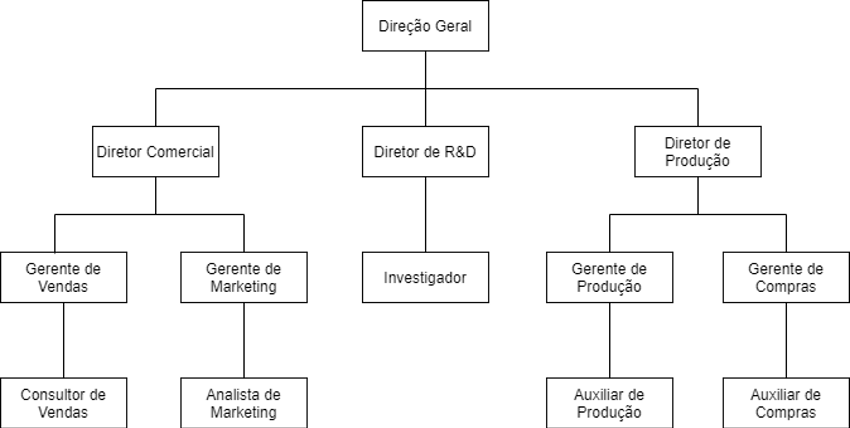
\includegraphics[scale=0.7]{Imagem1.png}\\
A NanoWave está dividida em 3 departamentos, cada um com funções diferentes e bastante específicas:
\begin{itemize}
    \item \textbf{Departamento Comercial} - Este é o departamento onde estão concentradas as ações que fazem todos os outros órgãos funcionarem devidamente e que está encarregue da parte estratégica da empresa. Como tal, o seu mau funcionamento prejudica todo o desempenho desta. Como objectivo final, este departamento foca-se no crescimento continuado da empresa.
    \item \textbf{Departamento de R\&D} - As funções deste departamento são completamente distintas das do resto da empresa. O seu papel é inovar e desenvolver os seus produtos e processos. Um bom departamento de R\&D é um departamento que permite à empresa manter-se relevante no mercado e ainda, se possível, fazê-la crescer.
    \item \textbf{Departamento de Produção} - Esta é a parte da empresa que está encarregue de converter matérias-primas nos NanoWaves que são posteriormente vendidos. Este departamento trabalha de forma a aumentar a eficiência da linha de montagem, de forma a estar sempre capaz de cumprir com as metas de produção exigidas pela administração da empresa. Por fim, para além da quantidade, também está incunbida de tentar sempre melhorar a qualidade dos produtos.
\end{itemize}

\subsection{Equipa de gestão e pessoal-chave }
Relativamente à equipa de gestão, podem-se destacar, pela sua importância e responsabilidade, os seguintes órgãos dentro da empresa:
\begin{itemize}
    \item \textbf{Direção Geral} - Este é o órgão que se encontra no topo da hierarquia da empresa. Devido às suas posições, as pessoas que fazem parte desta entidade têm a função mais complexa e crítica. É a Direção Geral que define o rumo estratégico geral da empresa. Isto pode ser alcançado através da:
    \begin{itemize}
        \item Seleção e nomeação das pessoas para os lugares de Diretor Comercial, R\&D e de Produção;
        \item Rescindimento das pessoas que ocupam os cargos referidos no ponto anterior;
        \item Aprovação dos orçamentos anuais;
        \item Prestação de contas às partes interessadas pelo desempenho e eficiência da empresa;
        \item Garantia da disponibilidade de recursos financeiros.
    \end{itemize}
    \item \textbf{Diretor Comercial} - Este é o elemento responsável pela estratégia comercial da empresa. Está relacionado com toda a parte de marketing e vendas e, por isso, a pessoa a quem este cargo pertence deve, preferencialmente, combinar um vasto conhecimento técnico da área com boas skills de marketing 
    \item \textbf{Gerente de Vendas} - Funciona como ajudante do Diretor Comercial, especialmente na parte das Vendas e a sua principal função é ser o responsável pelo cumprimento das metas destas. Tendo em conta o seu contacto próximo com os Consultores de Vendas e o facto de ser o superior hierárquico mais próximo destes, deverá possuir capacidades de liderança e de comunicação. Assim sendo, responsabiliza-se pelo desempenho da equipa de vendas relativamente às metas traçadas pelo Diretor Comercial.
    \item \textbf{Gerente de Marketing} - Este cargo é ocupado pela pessoa responsável pelas pesquisas de mercado e pelo desenvolvimento de estratégias que aumentem os resultados da empresa. Para tal, é necessário que o Gerente de Marketing seja alguém com um forte conhecimento do produto que é vendido e também dos produtos concorrentes. Apesar da elaboração de peças de publicidade não fazer parte das suas competências, deve saber aceitar ou recusar os anúncios feitos pelos Analistas de Marketing e Designers que estão sob a sua alçada, tendo em conta os objetivos definidos pelo Diretor Comercial.
    \item \textbf{Diretor de R\&D} - O profissional encarregue deste cargo é alguém que gere a inovação da empresa, ficando responsável pelo controlo, coordenação e pela pesquisa relativa aos:
    \begin{itemize}
        \item Produtos - Exploração de como o produto pode ser melhorado;
        \item Processos - Exploração de novos métodos e técnicas para criar produtos.
    \end{itemize}
    Um Diretor de R\&D competente é alguém que analisa as novas tendências do mercado e a procura deste, tentando sempre manter a sua empresa a par das tais tendências, de forma a mantê-la relevante no mercado atual.
    \item \textbf{Diretor de Produção} - É a pessoa incumbida pelo acompanhamento e avaliação da produção dos NanoWaves. Deve planear e supervisionar o fabrico do produto, enquanto assegura que são cumpridas as políticas de produção. Deve, portanto, ser alguém com um forte conhecimento de gestão de produção fabril e de gerência de índices de produtividade.
    \item \textbf{Gerente de Produção} - Gerente de Produção é o cargo de quem é responsável pelo cumprimento das metas de produção, sem nunca descurar:
    \begin{itemize}
        \item Padrões de Qualidade;
        \item Quantidade;
        \item Custos;
        \item Prazos estabelecidos.
    \end{itemize}
    Tendo em conta o seu contacto próximo com os Auxiliares de Produção que gere, é também ele que ajuda o Diretor de Produção a definir os requisitos de mão de obra e matérias-primas.
    \item \textbf{Gerente de Compras} - Esta pessoa ajuda o Diretor de Produção a gerir o setor de compras, analisando propostas e oportunidades, de forma a efetuar os melhores contratos. Na análise dos contratos, deve-se ter em conta:
    \begin{itemize}
        \item Preços;
        \item Condições de pagamento;
        \item Prazos de entrega.
    \end{itemize}
\end{itemize}

\subsection{Restante pessoal}
Já relativamente ao resto de todo o pessoal da empresa, há ainda que mencionar:
\begin{itemize}
    \item \textbf{Consultor de Vendas} - São aqueles que são responsáveis por toda a análise ao processo de vendas, com o intuito de tornar este processo não só mais eficiente como mais benéfico para a empresa. 
    \item \textbf{Analista de Marketing} - Analistas de Marketing e Designers formam juntos uma equipa que, sob a supervisão do Gerente de Marketing, se foca na análise das estratégias de Marketing anteriores da empresa e no estudo dos resultados destas, definindo novos planos de como publicitar a NanoWave.
    \item \textbf{Investigador} - Pessoa que, de uma forma sistemática, pratica um conjunto de atividades de inovação com o objetivo de desenvolver novos processos ou produtos e ainda de reinventar os já existentes.
    \item \textbf{Auxiliar de Produção} - Indivíduo que trabalha na linha de montagem e cuja função pode ser um misto entre operação das máquinas, manutenção e reparações fáceis destas e abastecimento da linha de produção. Por fim, pode também ajudar o Gerente de Produção no registo dos produtos e verificação da qualidade destes.
    \item \textbf{Auxiliar de Compras} - Profissional que, tal como o nome indica, presta auxílio nos processos de compra de matérias primas da parte da NanoWave. Esta ajuda pode passar pela emissão de documentos necessários às compras e pela confirmação de que os prazos e a qualidade são cumpridos.
\end{itemize}

\subsection{Subcontratação e consultoria}
Relativamente à subcontratação, pelo menos nesta parte inicial, a NanoWave não irá necessitar de nada mais do que uma transportadora que possa cumprir a expedição dos produtos para os clientes.\\
Já em relação à consultoria, não vemos razão para, neste momento, necessitar desta.


\part{Plano de financiamento}
\section{Investimento}
\subsection{Descrição dos investimentos necessários}
Tendo en conta a natureza da nossa empresa, foi planeado um custo inicial de 10 000 euros para a montagem do equipamento básico do escritório e da linha de montagem dos equipamentos, alocando metade deste valor para os seguintes anos de igual forma foram alocados 1500 euros anuais para equipamento administrativo. Ao terceiro ano está planeado a compra de um pequeno monovolume para a empresa, sendo utilizado até lá o transporte pessoal. \\ Para projetos de desenvolvimento, começamos com um investimento de 10000 no primeiro ano para o produto de entrada no mercado, alocando 20000 a partir do quarto ano anualmente para o desenvolvimento de novos produtos.
\subsection{Mapa de investimentos em valor}
\begin{table}[h]
\begin{tabular}{ | l | l | l | l | l | l | l | l | l | }
\hline
	Ano &  & 2021 & 2022 & 2023 & 2024 & 2025 & 2026 &  \\ \hline
	Activos fixos tangíveis &  &  &  &  &  &  &  &  \\ \hline
	Equipamento  Básico &  & 10000 & 5000 & 5000 & 5000 & 5000 & 5000 &  \\ \hline
	Equipamento de Transporte &  &  &  & 25000 &  &  &  &  \\ \hline
	Equipamento Administrativo &  & 1500 & 1500 & 1500 & 1500 & 1500 & 1500 &  \\ \hline
	Total Activos Fixos Tangíveis &  & 11500 & 6500 & 31500 & 6500 & 6500 & 6500 &  \\ \hline
	Activos Intangíveis &  &  &  &  &  &  &  &  \\ \hline
	Goodwill &  &  &  &  &  &  &  &  \\ \hline
	Projectos de desenvolvimento &  & 10000 &  &  & 20000 & 20000 & 20000 &  \\ \hline
	Programas de computador &  &  & &  &  &  &  &  \\ \hline
	Propriedade industrial &  &  &  &  &  &  &  &  \\ \hline
	Outros activos intangíveis &  & 10000 & 10000 & 10000 & 10000 & 10000 & 10000 &  \\ \hline
	Total Activos Intangíveis &  & 20000 & 10000 & 10000 & 30000 & 30000 & 30000 &  \\ \hline
	Total Investimento &  & 31500 & 16500 & 41500 & 36500 & 36500 & 36500 &  \\ \hline
	 &  &  &  &  &  &  &  &  \\ \hline
	 &  &  &  &  &  &  &  &  \\ \hline
	Valores Balanço &  & 2021 & 2022 & 2023 & 2024 & 2025 & 2026 &  \\ \hline
	Propriedades de investimento &  &  &  &  &  &  & 118 &  \\ \hline
	Activos fixos tangíveis &  & 10725  & 14750 & 36600 & 32525 & 27525 & 21750 &  \\ \hline
	Activos Intangíveis &  & 16667 & 16667 & 13333 & 23333 & 30000 & 30000 &  \\ \hline
	TOTAL &  & 27392 & 31417 & 49933 & 55858 & 57525 & 51750 &  \\ \hline
	 & \  & \  & \  & \  & \  & \  & \  & \  \\ \hline
\end{tabular}
\end{table}

\subsection{Calendário de execução do projeto}
Perante a projeção deste plano de financiamento é então apresentado um calendário de execução das futuras operações de desenvolvimento da NanoWave enquanto empresa:
\begin{table}[h]
\begin{tabular}{|l|l|l|}
\hline
                               & Data de início & Data de Conclusão \\ \hline
Estudo de plano de negócios    & 1/06/21          & 15/06/21             \\ \hline
Análise do Custo-Benefício     & 15/06/21          & 25/06/21             \\ \hline
Avaliação de impacto Ambiental & 15/06/21          & 25/06/21             \\ \hline
Estudos de conceção            & 26/06/21          & 20/07/21             \\ \hline
Estudos de R\&D                & 26/06/21          & 31/12/21             \\ \hline
Licença de desenvolvimento     & 01/07/21          & 30/07/21             \\ \hline
Fase Operacional               & 30/07/21          & ...            \\ \hline
Análise de entrada em mercados estrangeiros  & 01/06/22 & ... \\ \hline
Processo de Exportação & 01/01/23 & ... \\ \hline
Análise Resultados               & 01/03/22          & 01/04/22            \\ \hline
Novos Estudos de R\&D & 01/06/24 & ... \\ \hline
Nova Análise de Concepção  & 01/09/24 & 01/10/24 \\ \hline
Análise de Resultados do Produto & 01/06/25 & 01/07/25 \\ \hline

\end{tabular}
\end{table}
\section{Exploração}
\subsection{Pressupostos do estudo económico financeiro}
Foi definido um conjunto de pressupostos para a realização deste estudo económico. Consideramos que sejam relevantes referir os seguintes:
\begin{itemize}
    \item O período em análise é de 5 anos e 2 trimestres, iniciando-se em 2021 e acabando em 2026;
    \item O período de vendas inicia-se no último trimestre de 2021;
    \item A tabela de Gastos com Pessoal refere-se a 6 meses em 2021 (3 meses antes do início do período de vendas) visto que o processo de criação da empresa já estava em desenvolvimento;
    \item O prazo médio de recebimento e de pagamento é de 1 mês, enquanto que o de stockagem é de apenas 15 dias;
    \item Todas as taxas de IVA são a 23,00\%.
\end{itemize}
A maioria dos pressupostos pode ser analisado na seguinte tabela:
\begin{center}
    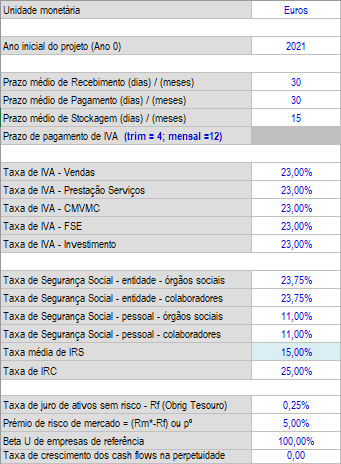
\includegraphics[scale=1.0]{images/pressupostos.png}
\end{center}

\subsection{Mapas de rendimentos de exploração}
Tendo em conta que o nanowave é um produto de nicho no mercado, a estrapolação de resultados de vendas foi realizada utilizando como referência alguns competidores e artigos idênticos existentes no mercado. Para a exportação tivemos em conta o aumento de público alvo, começando por países mais próximos e aumentando o alcance ao longo dos anos.\\Para além do produto inicial, foram incluídas nas vendas a projeção de um novo produto cuja entrada no mercado está prevista para 2024.
\begin{center}
    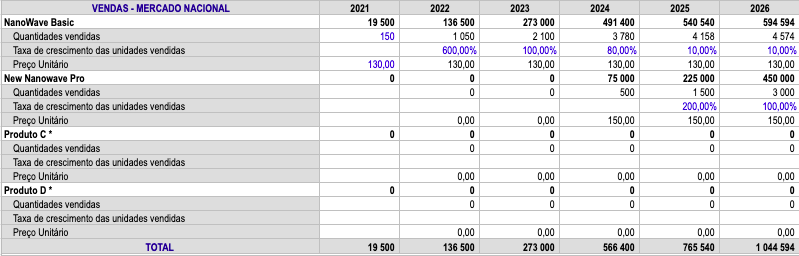
\includegraphics[scale=0.5]{images/vendas_nacionais.png}
\end{center}

\begin{center}
    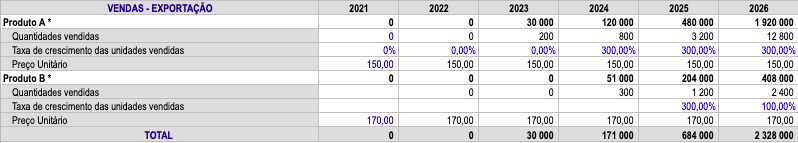
\includegraphics[scale=0.5]{images/vendas_exportacoes.png}
\end{center}

\subsection{Mapas de gastos de exploração}

A nível de gastos de exploração, tal como foi menciado previamente, a empresa produzirá a primeira versão do NanoWave com duas componentes maioritárias: as matérias-primas que incluem o metal e o plástico, à semelhança dos restantes microondas, sendo que neste caso acabe por ficar mais barato por causa das dimensões serem mais reduzidas; a componente elétrica da qual faz parte a bateria. Assim, para que o microondas possua a capacidade de permitir duas utilizações diárias de 2 minutos com uma potência de 1000 Watts cada, seria necessária uma bateria com uma capacidade a rondar os 269kJ. 
\par
Assim sendo, o custo de produção ronda os 90 euros(60 da bateria e 30 dos restantes materiais). O NanoWave é comercializado a um preço de 130 euros garantindo uma margem de lucro de aproximadamente 30\%.
\par
Planeia-se que para o ano de 2024, seja lançada uma nova versão do NanoWave com uma bateria melhorada e, desta forma, com um custo de produção mais elevado, que prefaça uma margem de lucro de 20\%.



\subsection{Conta de exploração /Demonstração Resultados}
Perante as projeções de gastos para a construção dos equipamentos chegou-se ao preço final de 130 euros para o NanoWave Basic. Este preço conta com uma margem de lucro na ordem dos 30\% para a empresa. Relativamente ao equipamento New Nanowave Pro o preço é previsto que seja 150 euros com uma margem de lucro na ordem dos 20\%, apesar das características finais do produto não terem sido ainda totalmente decididas. 
\begin{center}
    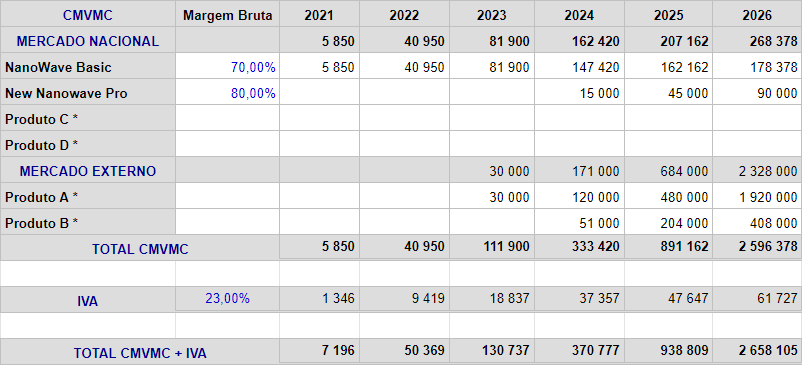
\includegraphics[scale=0.7]{images/cmvmc.png}
\end{center}
\section{Financiamento}
\subsection{Mapa descritivo das fontes de financiamento}
O financiamento inicial da empresa é feita pela entrada de 5000 euros do bolso de cada um dos seis fundadores da empresa fazendo um total de 30000 de entrada inicial de capital. Este capital será utilizado para aluguer do escritório e outros encargos, assim como a produção dos equipamentos iniciais. Nos anos futuros serão realizados dois pedidos de empréstimo ao banco de 20000 euros de cada vez. Este empréstimos serão pagos a 10 anos com uma taxa de juros de 5\%. A cada ano será realizada uma candidatura a bolsas de fundo perdido do estado.
\begin{center}
    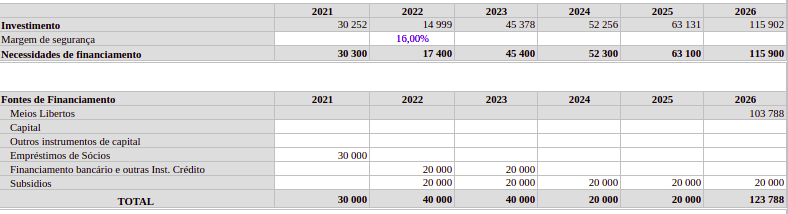
\includegraphics[scale=0.5]{images/financiamento.png}
\end{center}

\subsection{Orçamento de tesouraria}
\begin{center}
    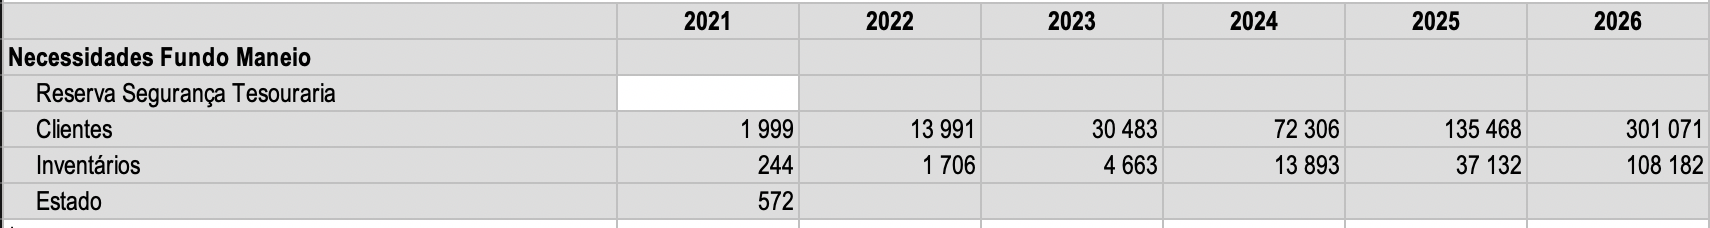
\includegraphics[scale=0.45]{images/tesouraria.png}
\end{center}

\subsection{Mapa de origem e aplicações de fundos}
\begin{center}
    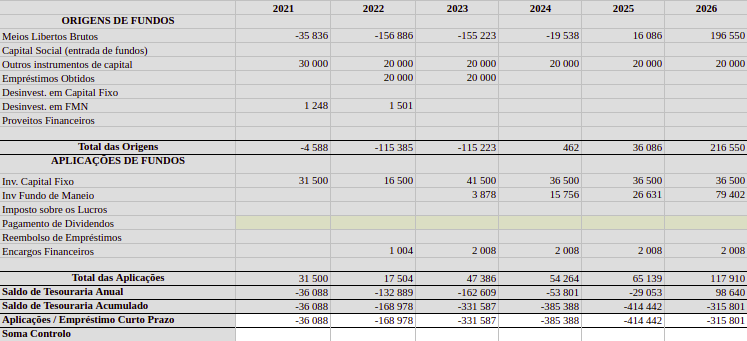
\includegraphics[scale=0.5]{images/planofinanciamento.png}
\end{center}

\subsection{Balanço previsional (documento de conclusão)}
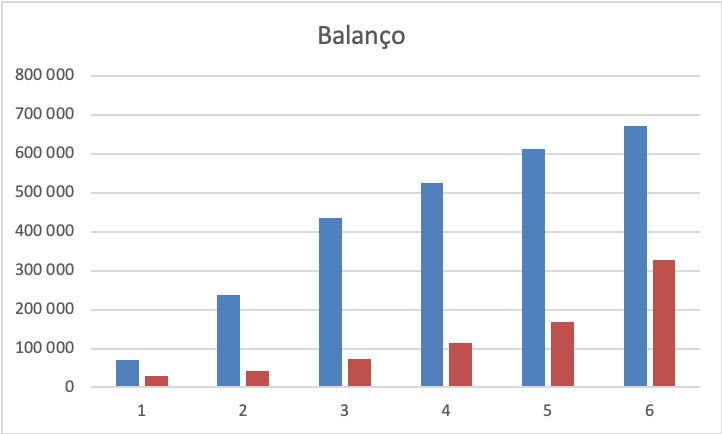
\includegraphics[scale=0.8]{images/balanço.png}\linebreak
O presente gráfico demonstra o crescimento do capital ativo (a vermelho) e passivo (a azul) no período em estudo.

O rácio de ativo para passivo é positivo, o que demonstra uma forte posição da empresa para possíveis imprevistos e investimentos.

\part{Análise de risco e viabilidade do projeto}
Após análise final do projeto, podemos analisar que, apesar do planeamento feito com todos os valores de gastos previstos arredondados substancialmente acima do valor real, tendo em conta que, da análise prevista a empresa apenas começa a ser lucrativa no quinto ano de desenvolvimento e da corrente instabilidade financeira do mercado, é difícil prever se haverá imprevistos que possam fazer com que esta data mude.

Sendo um produto de nicho, existe o risco de uma empresa maior que beneficie de vantagens competitivas (outras fontes de rendimento para subsidiar a alavancagem das vendas iniciais, preços favoráveis em publicidade, acesso a fornecedores que pratiquem preços mais baixos) possa entrar no nosso mercado e através da prática de preços mais baixos possibilitados pela sua escala inviabilizar o nosso projeto. 

Sendo que a manufatura das peças para o nosso produto será, inicialmente, feita por outras empresas, corremos o risco de ter dificuldades na gestão da supply chain de modo a conseguir ter stock suficiente para rapidamente enviar os produtos sem atingir níveis demasiado grandes de stock.

\part{Conclusão/Síntese}
Neste projeto foi possível desenvolver o estudo financeiro de uma empresa (NanoWave) criada no ano de 2021, empresa essa que se foca na produção de microondas portáteis. \par
Para a criação da NanoWave é necessário um investimento inicial de 31.500€ que iriam ser distribuídos por equipamentos básicos para se trabalhar na criação da empresa, pelos projetos de desenvolvimento e por ativos intangíveis. \par
Após a elaboração dos mapas financeiros e com base nestes, é esperado um capital positivo logo a partir do primeiro ano de produção (2021), mas apenas um cashflow positivo associado à venda dos microondas no último ano analisado (2026). \par
Tendo em conta os ainda baixos rendimentos da empresa no ano de 2026, consideramos pertinente referir que a NanoWave será, em princípio, nesse ano, uma empresa em forte crescimento, muito em virtude da sua expansão para o mercado externo. Um maior poder de compra em muitos países é uma das principais razões para um maior sucesso na venda do nosso produto que é, apesar tudo, caro para uma considerável parte do público alvo português. No entanto, acreditamos ser preferível a inclusão do nosso produto no mercado externo apenas no terceiro ano de produção de NanoWaves para a empresa ter tempo de se estabilizar e de observar o estado do mercado nessa altura. \par
Por fim, admitimos que os resultados atingidos por este estudo financeiro possam vir a ser ligeiramente diferentes daqueles que seriam obtidos caso a empresa fosse efetivamente criada. Estas diferenças podem estar relacionadas com uma pesquisa de mercado na qual não foi possível obter uma boa parte da informação que este trabalho requer. Para além de este ser um nicho de mercado, os dados que as empresas fornecem para o exterior são reduzidos e vagos, o que reduz a nossa capacidade de compreensão do atual estado do mercado.

%\begin{thebibliography}{}
%\bibitem{}

%\end{thebibliography}

\end{document}
